% Vietnamese translation for OI Public Library
% Source-PDF: IOI中国国家候选队论文/2007/day1/2.王晓珂《解析一类组合游戏》.pdf
\documentclass[11pt]{article}
\usepackage{oipl-vn}
\usepackage{tikz}

\newcommand{\SG}{\operatorname{SG}}
\newcommand{\mex}{\operatorname{mex}}
\newcommand{\xor}{\mathbin{\operatorname{xor}}}
\newcommand{\Oh}{\mathcal{O}}

\title{Phân tích đơn giản một lớp trò chơi tổ hợp}
\author{Wang Xiaoke\\Trường Trung học Nanshan Miên Dương, Tứ Xuyên}
\date{}

\begin{document}
\maketitle

\origtitle{A simple analysis of combinatorial games}
\sourcepath{IOI China candidate team papers / 2007 / day 1 / Wang Xiaoke}

\begin{abstract}
Nội dung chính của bài viết là các phương pháp phân tích trò chơi tổ hợp. Trước
khi giới thiệu những phương pháp ấy, ta sẽ trình bày các khái niệm liên quan.
Với mỗi phương pháp, bài viết kèm theo các ví dụ tương ứng để hỗ trợ việc hiểu
và vận dụng.
\end{abstract}

\paragraph{Từ khóa.}
Trò chơi tổ hợp; tổng của trò chơi; Nim; hàm Sprague--Grundy.

\section{Trò chơi tổ hợp và các khái niệm liên quan}

\subsection{Trò chơi tổ hợp}

Trò chơi là một khái niệm quen thuộc; thông thường nó chỉ các hoạt động mang
tính giải trí. Tuy vậy, nó cũng có thể có những hàm nghĩa khác như cạnh tranh
và tìm phương án tối ưu. Chẳng hạn cạnh tranh thương mại, đàm phán ngoại giao,
thậm chí chiến tranh, đều có thể được xem là trò chơi theo nghĩa ấy, dù chúng
không mấy vui vẻ.

Trong OI, rất nhiều bài toán được đặt ra từ trò chơi. Alice và Bob nổi tiếng
cũng vì lý do này. Trong các trò chơi ấy, trò chơi tổ hợp chiếm một phần rất
lớn. Thật ra trò chơi tổ hợp không xa lạ với chúng ta: đó là các trò chơi thỏa
mãn những điều kiện sau.

\begin{enumerate}
  \item Trò chơi có hai người tham gia.
  \item Tại mọi thời điểm trong quá trình chơi, trò chơi có một trạng thái xác
  định.
  \item Khi một người chơi thao tác, thao tác hợp lệ là đưa trò chơi từ trạng
  thái hiện tại sang một trạng thái khác; luật chơi quy định tập các trạng thái
  có thể đi tới từ mỗi trạng thái.
  \item Hai người chơi luân phiên thao tác.
  \item Khi trò chơi ở một trạng thái mà người chơi hiện tại không thể thao
  tác, trò chơi kết thúc. Khi ấy luật chơi quyết định thắng thua.
  \item Bất kể người chơi thao tác thế nào, trò chơi đều kết thúc sau hữu hạn
  bước, tức không có hòa.
  \item Người chơi biết toàn bộ thông tin về bản thân trò chơi và quá trình
  chơi, chẳng hạn luật chơi, các nước đi trước đó của mình và của đối thủ.
\end{enumerate}

Các trò chơi tổ hợp được xét trong bài viết này còn có thêm một ràng buộc công
bằng: luật thao tác của hai người chơi là như nhau.

Một trò chơi tổ hợp cũng có thể được biểu diễn bằng một đồ thị có hướng
\(G=(X,F)\), trong đó \(X\) là tập trạng thái của trò chơi, còn \(F(x)\) là tập
trạng thái có thể đi tới từ \(x\). Ở đây ta quy ước mọi trạng thái kết thúc đều
là trạng thái mà người chơi hiện tại thua. Nếu trong trò chơi gốc trạng thái
kết thúc là thắng, cần sửa mô hình đồ thị cho phù hợp với luật của bài toán.
Do không có hòa, đồ thị của trò chơi tổ hợp tất yếu là một đồ thị không chu
trình.

\subsection{Trạng thái thắng và trạng thái thua}

Trong trò chơi tổ hợp, một trạng thái thắng được định nghĩa là trạng thái mà
người chơi hiện tại có một chiến lược bảo đảm mình thắng bất kể đối thủ thao
tác thế nào. Ngược lại, nếu người chơi vừa đi trước đó có thể bảo đảm thắng,
thì trạng thái ấy là trạng thái thua.

Trong trò chơi tổ hợp, một trạng thái nếu không thua thì là thắng; điều này
hiển nhiên. Thông thường mục đích của ta khi phân tích trò chơi tổ hợp là phán
đoán một trạng thái là thắng hay thua, và nếu là thắng thì tìm chiến lược thắng.
Chỉ dựa vào định nghĩa trên chưa đủ để làm việc ấy. Các tính chất sau, cũng có
thể dùng để kiểm tra một phân hoạch trạng thái thắng--thua có đúng hay không,
nêu rõ một phương pháp truy hồi.

\begin{enumerate}
  \item Tính chất của trạng thái kết thúc do luật chơi quyết định.
  \item Với một trạng thái chưa kết thúc, nếu nó có thể đi tới một trạng thái
  thua nào đó thì nó là trạng thái thắng; nếu không, nó là trạng thái thua.
\end{enumerate}

Tuy tính chất này đúng với mọi trò chơi tổ hợp, nó không phải là vạn năng. Đôi
khi số trạng thái của trò chơi rất lớn, máy tính không thể xử lý trực tiếp; khi
đó ta phải mượn những phương pháp khác.

\subsection{Hàm Sprague--Grundy}

Đây là một hàm được định nghĩa trên các trạng thái của trò chơi tổ hợp. Ta dùng
\(g(x)\) để ký hiệu giá trị hàm tại trạng thái \(x\). Định nghĩa của nó là
\[
  g(x)=\mex\{g(y)\mid y\in F(x)\},
\]
tức giá trị của \(x\) là số tự nhiên nhỏ nhất khác với giá trị của mọi trạng
thái mà \(x\) có thể đi tới.

Độc giả cẩn thận hẳn đã nhận ra rằng \(g(x)=0\) khi và chỉ khi \(x\) là trạng
thái thua. Điều này rất dễ kiểm chứng từ định nghĩa.

\begin{enumerate}
  \item Khi \(x\) là trạng thái kết thúc, \(g(x)=0\), và nó là trạng thái thua.
  \item Khi \(x\) chưa kết thúc, nếu nó có thể đi tới một trạng thái thua thì
  \(g(x)>0\), nên \(x\) là trạng thái thắng.
  \item Nếu \(x\) chưa kết thúc và mọi trạng thái mà nó đi tới đều là trạng thái
  thắng, thì \(g(x)=0\), nên \(x\) là trạng thái thua.
\end{enumerate}

Định nghĩa dài dòng này thoạt nhìn dường như không có ý nghĩa, vì trực tiếp
phán đoán tính chất thắng thua của một trạng thái có vẻ tiện hơn nhiều so với
dùng hàm này. Nhưng thực tế trái với trực giác ấy: hàm SG là nền tảng của nhiều
phương pháp, và các tính chất của nó biến nó thành công cụ quan trọng khi phân
tích trò chơi tổ hợp.

\section{Tổng quan}

Trò chơi tổ hợp từ lâu là một chủ đề thú vị. Khi có máy tính, ta có thể phân
tích các trò chơi ấy dễ dàng hơn, và chúng dần đi vào các kỳ thi tin học. Vì
vậy nhu cầu nắm vững các phương pháp phân tích hợp lý cũng ngày càng tăng.

Ta luôn quan tâm liệu một trò chơi tổ hợp có chiến lược tất thắng hay không;
nếu có, phải thao tác thế nào để bảo đảm thắng. Đó là mục tiêu chính khi phân
tích trò chơi tổ hợp.

Trò chơi tổ hợp có nhiều quy luật phổ quát; đây là chìa khóa để phân tích
chúng. Làm thế nào để tận dụng các quy luật ấy? Với một trò chơi đặc biệt, làm
thế nào dùng tính đặc thù của nó để giúp việc phân tích trở nên thuận lợi?

Tác giả sẽ tổng kết quá trình phân tích nhiều trò chơi tổ hợp để rút ra một
hệ phương pháp hữu hiệu. Tuy nhiên, phương pháp nào cũng có giới hạn. Khi nắm
và vận dụng các phương pháp này, mong độc giả không để tư duy bị đóng khung
trong chúng; hãy xem chúng như nguồn gợi mở để rèn luyện tư duy, làm sắc bén
góc nhìn và mở rộng cách nghĩ.

Ba thủ đoạn cơ bản được giới thiệu trong bài viết là: phân rã trò chơi, quy
nạp, và biến đổi trò chơi.

\section{Phân rã trò chơi}

\subsection{Phân rã trò chơi và tổng của trò chơi}

Tổng của các trò chơi là trò chơi như sau: hai người chơi luân phiên thao tác
trên một số trò chơi con; mỗi lần thao tác có thể chọn tùy ý một trò chơi con
và thao tác trên trò chơi con đó; người đi nước cuối cùng thắng.

Trò chơi Nim là ví dụ kinh điển. Trong Nim, hai người luân phiên lấy đá từ một
số đống đá; mỗi lần có thể lấy tùy ý một số viên từ đúng một đống, nhưng phải
lấy ít nhất một viên; người lấy viên đá cuối cùng thắng. Nim nhiều đống được
tạo thành từ nhiều trò chơi Nim một đống, và mỗi lần thao tác chỉ được thao tác
theo luật của một trò chơi con.

Ta dùng
\[
  G=G_1+G_2+\cdots+G_n
\]
để biểu diễn tổng của các trò chơi, trong đó \(G_i=(X_i,F_i)\) là một trò chơi
tổ hợp đơn giản. Khi đó
\[
  X=X_1\times X_2\times\cdots\times X_n.
\]
Với \(x=(x_1,x_2,\ldots,x_n)\), ta có
\[
\begin{aligned}
F(x)
={}&F_1(x_1)\times\{x_2\}\times\cdots\times\{x_n\}\\
&{}\cup\{x_1\}\times F_2(x_2)\times\cdots\times\{x_n\}\\
&{}\cup\cdots\\
&{}\cup\{x_1\}\times\{x_2\}\times\cdots\times F_n(x_n).
\end{aligned}
\]

\subsection{Định lý Sprague--Grundy}

Tổng của trò chơi thường phức tạp hơn nhiều so với các trò chơi con. Chẳng hạn
với Nim, trò chơi con của nó khá đơn giản: ngoài trường hợp không còn đá là
thua, mọi trạng thái khác đều là trạng thái thắng. Nếu dùng \(x\) để biểu diễn
trạng thái có \(x\) viên đá, thì trường hợp một đống rất dễ hiểu. Nhưng với
nhiều đống, số trạng thái tăng vọt và quan hệ giữa các trạng thái cũng phức
tạp hơn nhiều, khiến việc phân tích trở nên khó khăn.

Ta biết một trạng thái là trạng thái thua khi và chỉ khi giá trị SG của nó bằng
0; giá trị SG của mọi trạng thái hoàn tất việc phân hoạch thắng--thua. Định lý
Sprague--Grundy dùng để tìm giá trị SG của những trò chơi dạng tổng như vậy.

Quy luật của trò chơi kinh điển Nim thật ra rất đơn giản. Với \(n\) đống đá,
giả sử đống thứ \(i\) có \(x_i\) viên đá, trạng thái là thua khi và chỉ khi
\[
  x_1\xor x_2\xor\cdots\xor x_n=0.
\]
Vì những trạng thái này là trạng thái thua, giá trị SG của chúng cũng bằng 0.
Đến đây, nội dung định lý gần như có thể đoán ra.

\paragraph{Định lý Sprague--Grundy.}
Với \(G=G_1+G_2+\cdots+G_n\),
\[
  g_G(x_1,x_2,\ldots,x_n)=
  g_1(x_1)\xor g_2(x_2)\xor\cdots\xor g_n(x_n).
\]

\paragraph{Chứng minh.}
Phép toán xor có một số tính chất quan trọng giống phép cộng; ở đây ta giới
thiệu những tính chất cần dùng. Nếu \(a\xor b=c\), thì bit thứ \(i\) trong biểu
diễn nhị phân của \(c\) là tổng modulo 2 của bit thứ \(i\) của \(a\) và \(b\).
Phép xor có tính kết hợp và giao hoán. Ngoài ra,
\[
  a\xor a=0,\qquad a\xor 0=a,
\]
và khi biết hai trong ba giá trị \(a,b,c\) thỏa \(a\xor b=c\), giá trị còn lại
được xác định duy nhất.

Đặt
\[
  b=g_1(x_1)\xor g_2(x_2)\xor\cdots\xor g_n(x_n).
\]
Theo định nghĩa của \(\mex\), chỉ cần chứng minh hai mệnh đề sau.

\begin{enumerate}
  \item Với mọi \(a\in\mathbb{N}\) và \(a<b\), tồn tại \(x'\in F(x)\) sao cho
  \(g_G(x')=a\).
  \item Với mọi \(x'\in F(x)\), ta có \(g_G(x')\ne b\).
\end{enumerate}

Chứng minh mệnh đề 1. Đặt \(d=a\xor b\), và gọi \(k\) là bit cao nhất bằng 1
trong biểu diễn nhị phân của \(d\). Vì \(a<b\), tại bit \(k\), \(b\) có bit 1
còn \(a\) có bit 0. Do đó tồn tại một chỉ số \(i\) sao cho bit thứ \(k\) của
\(g_i(x_i)\) bằng 1. Khi ấy
\[
  g_i(x_i)\xor d < g_i(x_i).
\]
Theo định nghĩa của hàm SG, tồn tại \(x_i'\in F_i(x_i)\) sao cho
\[
  g_i(x_i')=g_i(x_i)\xor d.
\]
Vì \(b\xor d=a\), ta có
\[
\begin{aligned}
a
&=g_1(x_1)\xor\cdots\xor g_i(x_i)\xor d\xor\cdots\xor g_n(x_n)\\
&=g_G(x_1,\ldots,x_i',\ldots,x_n).
\end{aligned}
\]
Mà \((x_1,\ldots,x_i',\ldots,x_n)\in F(x)\), nên mệnh đề 1 được chứng minh.

Chứng minh mệnh đề 2. Giả sử ngược lại rằng tồn tại \(x'\in F(x)\) sao cho
\(g_G(x')=b\). Khi đó chỉ có một thành phần thay đổi, tức
\[
  x'=(x_1,\ldots,x_i',\ldots,x_n)
\]
với \(x_i'\in F_i(x_i)\). Từ \(g_G(x')=b=g_G(x)\) suy ra
\[
  g_i(x_i')=g_i(x_i),
\]
mâu thuẫn với định nghĩa của hàm SG: một trạng thái không thể đi tới trạng thái
có cùng giá trị SG. Vậy mệnh đề 2 được chứng minh.

Trong chứng minh trên có dùng kết quả cho các trạng thái con, nên lập luận đầy
đủ cần được đặt trong quy nạp toán học trên thứ tự topo của đồ thị trò chơi.

Như vậy, không phải lúc nào hàm SG cũng khó tìm hơn trạng thái thua. Phân rã
một trò chơi nghĩa là xem nó như tổng của vài trò chơi và dùng kết quả phân
tích từng trò chơi riêng lẻ để nghiên cứu toàn bộ trò chơi. Hầu như mọi trò
chơi con đều đơn giản hơn tổng của chúng; do đó khi đối mặt với phần lớn các
tổng trò chơi phức tạp, phương pháp phân rã thường giải quyết được vấn đề.

\subsection*{Ví dụ 1: A Funny Stone Game}

\begin{center}
ACM ICPC 2006 Asia Regional Contest, Beijing
\end{center}

David chơi một trò chơi với đá. Có \(n\) đống đá, đánh số từ \(0\) đến \(n-1\).
Hai người chơi luân phiên lấy đá. Ở mỗi lượt, người chơi chọn ba đống đá
\(i,j,k\), trong đó \(i<j\), \(j\le k\), và đống \(i\) có ít nhất một viên đá;
sau đó lấy một viên đá từ đống \(i\), rồi bỏ thêm một viên vào mỗi đống \(j\)
và \(k\). Nếu \(j=k\), tức là bỏ hai viên vào đống \(k\). Người đầu tiên không
thể lấy đá sẽ thua. Hãy lập trình giúp David.

Số đống đá không vượt quá 23, và mỗi đống có không quá 1000 viên đá.

\paragraph{Input.}
Dữ liệu vào gồm nhiều bộ dữ liệu. Mỗi bộ gồm hai dòng: dòng thứ nhất là số
nguyên \(n\), dòng thứ hai chứa \(n\) số nguyên \(S_0,\ldots,S_{n-1}\), biểu
diễn số đá trong từng đống. Dữ liệu kết thúc bằng một dòng chứa số 0.

\paragraph{Output.}
Với mỗi bộ dữ liệu, in một dòng. Định dạng là
\[
  \texttt{Game t: i j k},
\]
trong đó \(t\) là số thứ tự bộ dữ liệu, còn \(i,j,k\) biểu diễn một nước mở đầu
bảo đảm David thắng. Nếu có nhiều phương án, in bộ nhỏ nhất theo thứ tự từ điển.
Nếu không có phương án như vậy thì \(i,j,k\) đều bằng \(-1\).

\paragraph{Phân tích.}
Nhìn trò chơi từ một góc độ khác, ta có thể xem mỗi viên đá là một đống đá. Nếu
viên đá ấy nằm trong đống thứ \(p\), thì kích thước của đống mà nó đại diện là
\(n-1-p\). Khi đó một thao tác trở thành: lấy đi một đống không có kích thước
0, rồi đặt vào hai đống có kích thước nhỏ hơn nó, có thể là 0. Như vậy ta thu
được một trò chơi khác. Ta làm thế vì trò chơi sau khi chuyển đổi rất giống
trò chơi kinh điển \emph{take-and-break}.

Do các viên đá không ảnh hưởng lẫn nhau, trò chơi có thể xem là tổng của nhiều
trò chơi chỉ có một đống.

Trước hết phân tích trò chơi con. Để tính giá trị SG của trạng thái \(x\) trong
trò chơi con, ta cần giá trị SG của các trạng thái kế tiếp. Phần lớn trạng thái
kế tiếp của trò chơi con chứa hai đống, nhưng cả hai đều có kích thước nhỏ hơn
\(x\). Khi đã biết giá trị hàm cho các trạng thái có kích thước nhỏ hơn \(x\),
ta có thể dùng định lý SG để tính giá trị của mọi trạng thái kế tiếp.

Dùng \((p)\) để biểu diễn trạng thái chỉ còn một đống kích thước \(p\), và
\((p,q)\) để biểu diễn trạng thái còn hai đống kích thước lần lượt là \(p,q\).
Khi ấy
\[
  g(p,q)=g(p)\xor g(q),
\]
và
\[
  g(x)=\mex\{g(p)\xor g(q)\mid 0\le p<x,\ 0\le q<x\}.
\]

Áp dụng kết luận trên, ta có thể truy hồi để tính giá trị SG của mọi trạng thái
trong trò chơi con. Sau đó dùng định lý SG để tính giá trị SG của mọi trạng
thái trong tổng trò chơi. Nếu \(\SG=0\), David không thể bảo đảm thắng; ngược
lại, David có thể thắng. Về chiến lược, chỉ cần chọn một thao tác sao cho trạng
thái để lại có giá trị SG bằng 0.

\paragraph{Độ phức tạp thời gian.}
Thuật toán trên gồm \(\Oh(n)\) phép tính giá trị SG, mỗi phép tính nhiều nhất
tốn \(\Oh(n^2)\). Việc phán đoán trạng thái thắng cần \(\Oh(\sum S_i)\), còn
tìm chiến lược tối ưu cần \(\Oh(n^3)\). Tổng hợp lại, độ phức tạp thời gian là
\[
  \Oh\!\left(n^3+\sum_i S_i\right).
\]

\section{Quy nạp}

Quy nạp cũng là một phương pháp thường gặp khi phân tích trò chơi tổ hợp. Nhờ
quy nạp, ta có thể hoàn tất phân tích rất nhiều trạng thái trong thời gian
ngắn. Chẳng hạn với Nim một đống, từ cơ sở truy hồi đơn giản ta có thể quy nạp
ra rằng trạng thái kích thước \(x\) có giá trị SG bằng \(x\), và \(x\) thua khi
và chỉ khi \(x=0\). Vì kết quả quy nạp thường đơn giản ngoài dự đoán, tôi tin
rằng khi tự phân tích trò chơi tổ hợp, độc giả sẽ tự nhiên dùng phương pháp này.

Đối tượng được quy nạp không chỉ là các trạng thái thua quen thuộc mà còn có
thể là hàm SG vừa giới thiệu.

Thông thường, cơ sở để ta đưa ra quy nạp là đặc điểm của các tình huống đơn
giản trong trò chơi. Tuy nhiên, những tình huống đơn giản trong trò chơi chỉ
gợi ý được một phần. Đôi khi ta phải đưa ra phỏng đoán dựa trên kinh nghiệm
hơn là trên dữ kiện đã có. Nhiều trò chơi vừa giống vừa khác các trò chơi kinh
điển; tìm ra điểm tương tự trong mô hình và đưa ra phỏng đoán hợp lý đôi khi
trực tiếp và hiệu quả hơn so với quy nạp từ dữ liệu thô.

\subsection*{Ví dụ 2: Staircase Nim}

Đây là một trò chơi tổ hợp kinh điển. Ban đầu có nhiều đồng xu phân bố tùy ý
trên cầu thang. Có tổng cộng \(n\) bậc, đánh số từ mặt đất lên trên là
\(0,1,\ldots,n\). Mỗi lần thao tác, người chơi có thể chuyển tùy ý một số đồng
xu, nhưng ít nhất một đồng, từ bậc \(j\) với \(1\le j\le n\) xuống bậc
\(j-1\). Hai người chơi luân phiên thao tác; người chuyển đồng xu cuối cùng
xuống đất thắng.

\paragraph{Phân tích.}
Điểm khác biệt giữa bài toán này và Nim là những đồng xu bị chuyển không bị bỏ
đi, mà được đưa vào một đống khác. Ta cân nhắc liệu có thể loại bỏ một phần cầu
thang khỏi phạm vi xét hay không. Các bậc lẻ chỉ có thể đẩy đồng xu xuống bậc
chẵn, và tương tự, đồng xu trên bậc chẵn chỉ có thể bị đẩy xuống bậc lẻ. Nếu
chỉ xét Nim trên các bậc lẻ và xem các bậc chẵn chỉ như vật chứa, trò chơi trở
thành Nim. Khi đồng xu trên bậc chẵn cũng có thể được chuyển ra, liệu ta vẫn
có thể dùng phương pháp Nim để phán đoán trạng thái thua hay không?

Gọi điều kiện A là ``xor Nim của số đồng xu trên các bậc lẻ bằng 0''. Trạng thái
kết thúc thỏa điều kiện A. Mọi trạng thái thỏa điều kiện A đều chỉ có thể đi
tới trạng thái không thỏa điều kiện A. Mọi trạng thái không thỏa điều kiện A
đều có thể đi tới một trạng thái thỏa điều kiện A, theo đúng lập luận của Nim.
Vì vậy một trạng thái là trạng thái thua khi và chỉ khi nó thỏa điều kiện A.

\subsection*{Ví dụ 3: Lật đồng xu}

Đây cũng là một trò chơi tổ hợp kinh điển. Trên một đường thẳng có một hàng
đồng xu, một số mặt sấp và một số mặt ngửa. Hai người chơi luân phiên lật đồng
xu. Khi lật, trước hết chọn một đồng xu đang ngửa mặt để lật;
sau đó, nếu muốn, có thể chọn thêm một đồng xu ở bên trái nó để lật. Người
thực hiện nước lật làm cho tất cả đồng xu đều úp mặt sấp sẽ thắng.

\begin{center}
\begin{tikzpicture}[x=0.46cm,y=0.42cm]
  \foreach \i/\v in {1/T,2/H,3/T,4/T,5/H,6/T,7/T,8/T,9/H,10/H,11/T,12/H,13/T} {
    \node[font=\large] at (\i,1) {\v};
    \node[font=\small] at (\i,0) {\i};
  }
  \draw[blue!70,thick,rounded corners] (1.62,-0.35) rectangle (2.38,1.42);
  \draw[blue!70,thick,rounded corners] (11.58,-0.35) rectangle (12.42,1.42);
  \draw[->,blue!70,thick,bend left=18] (2,1.65) to node[above,font=\small]
    {lật cùng lúc} (12,1.65);
\end{tikzpicture}\\[-0.2em]
{\small Hình 1: trạng thái của trò lật đồng xu; lật đồng thời hai đồng xu ở
vị trí 2 và 12 là một thao tác hợp lệ.}
\end{center}

\paragraph{Phân tích.}
Dựa trên tư tưởng biến đổi, nếu xem một đồng xu mặt ngửa ở vị trí \(i\) như
một đống đá kích thước \(i\), ta có thể thấy trò chơi này tương tự Nim. Tuy
nhiên, nhiều thao tác hợp lệ trong Nim không thể thực hiện trong trò chơi này.
Ví dụ ở trạng thái trong hình 1, ta không thể lấy 5 viên từ một đống kích thước
10. Nhưng nếu ta lật đồng thời các vị trí 10 và 5, trạng thái thu được có cùng
giá trị SG với thao tác ``lấy 5 viên từ 10'' trong Nim. Vì vậy ta phỏng đoán
rằng giá trị SG của trạng thái trong trò chơi này bằng giá trị SG của trạng
thái Nim tương ứng. Trên thực tế, dù trò chơi này không thể thực hiện mọi thao
tác của Nim, tập giá trị SG của các trạng thái nó có thể đi tới lại trùng với
tập tương ứng trong Nim. Do đó giá trị SG của nó đúng là giống Nim.

\section{Biến đổi trò chơi}

Trong thực tế, nhiều trò chơi ẩn giấu các đặc điểm cần thiết cho phân tích dưới
một hình thức nào đó; một số trò chơi có trạng thái chứa nhiều yếu tố và quan
hệ rất phức tạp. Khi gặp những tình huống khiến ta không biết bắt đầu từ đâu,
ta nên nghĩ đến việc biến đổi trò chơi.

Bài viết giới thiệu hai phương pháp: thứ nhất là biến đổi hình thức của trò
chơi, tức biến đổi tương đương; thứ hai là biến đổi không tương đương trạng
thái dưới một số điều kiện.

\subsection{Biến đổi tương đương}

Cùng một trò chơi tổ hợp thường có nhiều hình thức biểu hiện khác nhau. Chẳng
hạn trò chơi \emph{take-and-break} được nhắc trong ví dụ 1 có thể chuyển thành
một trò chơi đá có hình thức hoàn toàn khác, chỉ cần sửa ví dụ 1 một chút là
có thể khiến nó tương đương với \emph{take-and-break}. Với cùng một trò chơi,
từ các góc nhìn khác nhau, ta quan sát được các tính chất khác nhau. Ví dụ 1 ở
hình thức ban đầu rất khó thể hiện bản chất ``tổng của trò chơi''; sau một phép
biến đổi khéo léo, tính chất ấy hiện rõ.

\subsection*{Ví dụ 4: Game}

\begin{center}
POI 2003/2004, vòng I
\end{center}

Trò chơi được tiến hành trên một bàn \(m\times 1\). Một số ô đơn vị trên bàn có
đặt một quân. Hai người chơi luân phiên di chuyển quân. Khi di chuyển, chọn một
quân và đặt nó vào ô trống gần nhất ở bên phải; nếu không tồn tại ô như vậy,
thì ném quân đó đi. Người ném quân cuối cùng thắng.

\begin{center}
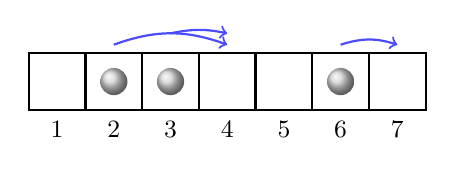
\begin{tikzpicture}[x=0.72cm,y=0.72cm]
  \foreach \i in {1,...,7} {
    \draw[thick] (\i-1,0) rectangle (\i,1);
    \node[font=\small] at (\i-0.5,-0.35) {\i};
  }
  \foreach \i in {2,3,6} {
    \shade[ball color=gray!35] (\i-0.5,0.5) circle (0.24);
  }
  \draw[->,blue!70,thick,bend left=20] (1.5,1.15) to (3.5,1.15);
  \draw[->,blue!70,thick,bend left=12] (2.5,1.35) to (3.5,1.35);
  \draw[->,blue!70,thick,bend left=18] (5.5,1.15) to (6.5,1.15);
\end{tikzpicture}\\[-0.2em]
{\small Hình 2: bàn \(m=7\); có thể chuyển quân ở ô 2 hoặc 3 sang ô 4, hoặc
quân ở ô 6 sang ô 7.}
\end{center}

Với trạng thái cho trước, hãy xuất số nước đi đầu tiên bảo đảm người đi trước
thắng.

\paragraph{Input.}
Dòng đầu nhập \(m,n\), trong đó \(m\) là kích thước bàn và \(n\) là số quân.
Dòng thứ hai gồm \(n\) số biểu diễn vị trí của từng quân.

\paragraph{Output.}
In một dòng duy nhất: số chiến lược bảo đảm người đi trước thắng.

\paragraph{Phân tích.}
Trước hết, các quân ảnh hưởng lẫn nhau, nên rất khó xem trò chơi là tổng của
các trò chơi con. Trạng thái nhiều, quan hệ phức tạp, và rất khó trực tiếp tìm
các trạng thái thua. Ta xét biến đổi trò chơi. Sau nhiều lần thử, có thể biến
đổi như sau: xem khoảng giữa mỗi ô trống và ô trống gần nhất bên trái nó là một
bậc cầu thang; phần bên phải ô trống cuối cùng được xem là mặt đất; số quân
trong mỗi đoạn không gian là số đồng xu trên bậc cầu thang tương ứng. Khi đó
trò chơi hoàn toàn tương đương với Staircase Nim.

\paragraph{Nhận xét.}
Nếu không biến đổi thành công ví dụ này, quá trình phân tích của ta sẽ rất dễ
gây nản lòng. Khi đối mặt với trò chơi tổ hợp, quan sát nó từ các góc nhìn khác
nhau, tức biến đổi nó, nên là một trong những thủ đoạn cơ bản. Các trò chơi
lấy đá hoặc lấy đồng xu là những trò ta quen thuộc nhất, nên có thể xem là lựa
chọn đầu tiên để thử biến đổi. Dù biến đổi theo cách nào, mục tiêu vẫn là đào
sâu bản chất và đặc điểm của trò chơi.

\subsection{Biến đổi không tương đương}

Khi phân tích trò chơi tổ hợp, chỉ cần biết giá trị SG là đủ. Nếu cứ biến đổi
trò chơi một cách nguyên xi, giữ bản chất trò chơi hoàn toàn không đổi, liệu
có hơi lãng phí hay không?

Vì ta chỉ cần giá trị SG, có thể kỳ vọng rằng trong khi bảo đảm giá trị SG của
trạng thái không đổi, ta thực hiện một phép biến đổi không tương đương để đơn
giản hóa trạng thái phức tạp thành trạng thái mộc mạc nhất, rồi giải quyết dễ
dàng.

\subsection*{Ví dụ 5: Got Root?}

\begin{center}
IPSC 2003
\end{center}

Một ngày nọ, Alice và Bob phát hiện một bụi cây kỳ lạ: các cành của nó sau khi
phân nhánh lại có thể hợp lại; lạ hơn nữa, không chỉ các nhánh xuất phát từ
cùng một điểm mới có thể hợp lại, mà ngay cả hai cành có điểm phân nhánh rất
xa nhau cũng có thể mọc dính vào nhau. Theo cách nhìn của chúng ta, nó có thể
được trừu tượng hóa thành một đồ thị vô hướng, trong đó có một đỉnh duy nhất
là gốc.

Họ cho rằng đây là vật liệu tuyệt vời để chơi trò chơi, nên dự định chơi trò
chặt cành trên cái cây này. Luật như sau.

\begin{enumerate}
  \item Hai người luân phiên chặt một cành, tức một cạnh trên đồ thị. Mỗi lần
  chặt một cạnh, phần không còn nối với gốc sẽ bị bỏ đi.
  \item Người chặt cành cuối cùng thắng.
\end{enumerate}

Alice đi trước. Với đồ thị vô hướng cho trước, hãy xuất tên người thắng.

\paragraph{Phân tích.}
Đã muốn biến đổi thì ta cần có một mục tiêu: một trạng thái đơn giản hơn. Trước
hết ta xét trường hợp đồ thị là cây xem có đơn giản hơn không. Sau phân tích
sơ bộ, trạng thái dạng cây vẫn khó cho kết luận trực tiếp; nó còn cần đơn giản
hóa thêm. Ta xét tiếp trường hợp đồ thị là một chuỗi dài. Lúc này cuối cùng có
kết quả thỏa đáng: bài toán trở thành Nim một đống điển hình, và có thể trực
tiếp tính giá trị SG.

Vậy làm thế nào biến đồ thị thành chuỗi? Ta thực hiện theo hai bước: trước hết
biến đồ thị thành cây, rồi biến cây thành chuỗi. Toàn bộ quá trình giữ nguyên
giá trị SG của trạng thái.

Làm bước thứ hai trước. Khi chỉ có một điểm phân nhánh, đây là một Nim đơn
giản: có thể biến nó thành một chuỗi đơn có độ dài bằng xor độ dài của từng
chuỗi nhánh. Với một cây phức tạp hơn, ta phỏng đoán rằng bắt đầu từ các đầu
mút và làm như vậy, mỗi nơi phân nhánh có thể được gộp thành một chuỗi duy
nhất có độ dài bằng xor của các chuỗi con, mà không thay đổi giá trị SG của
toàn bộ trạng thái.

Cách gộp này có thể mở rộng thành kết luận tổng quát hơn: với hai cây bất kỳ
\(H_1,H_2\), nếu giá trị SG của trò chặt cành trên chúng bằng nhau, thì khi gắn
chúng vào hai đỉnh tương ứng của hai đồ thị giống nhau, hai đồ thị mới thu
được cũng có cùng giá trị SG.

Chứng minh kết luận này có tính điển hình cho các mệnh đề ``hai trạng thái có
cùng giá trị SG''. Gọi hai đồ thị sinh ra là \(G_1\) và \(G_2\). Trước hết
chứng minh trong trò chơi \(G_1+G_2\), người đi sau có chiến lược thắng. Nếu
người thứ nhất chặt một cạnh không thuộc \(H_1\) hoặc \(H_2\), người thứ hai
chặt cạnh tương ứng trong thành phần còn lại. Nếu người thứ nhất chặt một cạnh
thuộc \(H_1\) hoặc \(H_2\), người thứ hai chặt một cạnh thích hợp trong cây có
giá trị SG cao hơn giữa \(H_1,H_2\), sao cho hai phần còn lại có giá trị SG
bằng nhau. Do đó \(g(G_1+G_2)=0\), tức \(g(G_1)=g(G_2)\).

Tiếp theo cần biến đồ thị thành cây.

Điểm khác nhau giữa đồ thị và cây là đồ thị có chu trình còn cây thì không.
Tư tưởng mộc mạc nhất để biến đồ thị thành cây là lần lượt co các chu trình
trong đồ thị thành một điểm. Vậy các cạnh liên quan xử lý thế nào? Cạnh trong
đồ thị là đối tượng thao tác của trò chơi, nên tốt nhất là giữ lại tất cả
chúng. Về đầu mút, nếu chúng đã bị gộp lại, cạnh đó trở thành một vòng tự nối.

Ta hy vọng phép biến đổi này giữ nguyên giá trị SG. Chứng minh kết luận này
tương đối dài, nên bài viết không trình bày ở đây mà đưa vào phụ lục.

Tuy vậy, thao tác này cuối cùng sẽ để lại rất nhiều vòng tự nối. Không khó thấy
một vòng tự nối tương đương với một chuỗi đơn độ dài 1. Như vậy ta đã có cơ sở
lý thuyết cho phép biến đổi từ đồ thị sang cây.

\paragraph{Thuật toán.}
Từ các kết luận trên, ta có thể thiết kế thuật toán biến đồ thị thành một chuỗi
đơn mà giá trị SG không đổi. Trong đồ thị vô hướng, có một cách phân hoạch sao
cho trong mỗi tập, xóa bất kỳ một cạnh nào vẫn giữ liên thông, còn giữa các tập
thì tồn tại cầu. Mỗi tập có thể được co thành một điểm nhờ thao tác co chu
trình, kèm theo một đống vòng tự nối tại chính điểm đó. Thuật toán có thể co
đồ thị theo cách này trong \(\Oh(e)\) thời gian, rồi dùng \(\Oh(n)\) thời gian
để hoàn tất phép biến đổi sang cây và chuỗi. Toàn bộ quá trình giữ nguyên giá
trị SG của trạng thái. Sau khi biến đổi xong, bài toán trở nên rất dễ giải.

Độ phức tạp thời gian của thuật toán là \(\Oh(e)\).

\section{Kết luận}

Sau khi lần lượt trình bày ba phương pháp, tác giả hy vọng độc giả có được
nhận thức tương đối toàn diện về trò chơi tổ hợp và quá trình phân tích chúng,
từ đó có thể vận dụng linh hoạt trong thi đấu.

Nội dung của trò chơi tổ hợp rất rộng; những phương pháp này vẫn không giải
quyết được nhiều vấn đề. Độc giả có hứng thú không nên bó buộc trong phạm vi
bài viết, mà có thể tìm hiểu thêm về trò chơi tổ hợp từ các sách liên quan.

Giải trò chơi tổ hợp không khó; điều quan trọng là mở rộng tri thức, thường
xuyên tổng kết, vận dụng linh hoạt và phát triển các phương pháp đã biết.

\section*{Lời cảm ơn}

Xin cảm ơn thầy Ye Shifu và thầy Liu Rujia vì sự giúp đỡ và chỉ dẫn. Xin cảm
ơn các bạn He Sen và Gu Nan vì những góp ý quý báu.

\section*{Tài liệu tham khảo}

\begin{itemize}
  \item \emph{Game Theory}, Ferguson.
\end{itemize}

\appendix

\section{Chứng minh nguyên lý dung hợp}

Phần này trích từ website chính thức của IPSC. Trong đó, \emph{colon
principle} chỉ kết luận dùng để biến cây thành chuỗi.

\paragraph{Chứng minh nguyên lý dung hợp.}
Giả sử ngược lại. Lấy một phản ví dụ có số cạnh ít nhất; nếu có nhiều phản ví
dụ như vậy, chọn phản ví dụ có số đỉnh ít nhất. Gọi đồ thị ấy là \(G\). Ta có
thể suy ra các sự kiện sau về \(G\).

\begin{itemize}
  \item Với hai đỉnh tùy ý \(x,y\) nằm trên một chu trình nào đó của \(G\), nếu
  dung hợp \(x\) và \(y\), giá trị SG của \(G\) sẽ thay đổi; nếu không, ta đã có
  một phản ví dụ nhỏ hơn.

  \item Khi xóa đỉnh 1, \(G\) vẫn liên thông; nếu không, một thành phần liên
  thông cùng với đỉnh 1 sẽ tạo thành phản ví dụ nhỏ hơn.

  \item Không có cặp đỉnh nào trong \(G\) được nối bởi ba đường đi rời cạnh.
  Giả sử ngược lại rằng hai đỉnh \(x,y\) trong \(G\) được nối bởi ba đường đi
  rời cạnh. Dung hợp \(x\) và \(y\), thu được đồ thị \(H\). Đồ thị \(H\) phải
  có giá trị SG khác \(G\). Vì giá trị SG của \(G\) và \(H\) khác nhau, nên
  \(G+H\) là vị thế thắng cho người đến lượt đi. Ta thực hiện một nước thắng.
  Sau đó ta đáp lại nước tiếp theo bằng cách xóa cạnh tương ứng trong thành
  phần còn lại. Ví dụ nếu nước thắng cắt một cạnh trong \(G\), ta cắt ``cùng''
  cạnh ấy trong \(H\). Ta thu được vị thế \(G'+H'\), vốn lại phải là vị thế
  thắng. Chú ý rằng trong \(G'\), hai đỉnh \(x,y\) vẫn được nối bởi ít nhất hai
  đường đi rời cạnh. Tuy nhiên \(G'\) nhỏ hơn \(G\), nên nguyên lý dung hợp
  đúng với \(G'\). Ta có thể dung hợp \(x\) và \(y\) mà không làm đổi giá trị SG
  của \(G'\). Nhưng dung hợp \(x\) và \(y\) trong \(G'\) chính là \(H'\). Suy ra
  \(G'\) và \(H'\) có cùng giá trị SG. Nói cách khác, \(G'+H'\) là vị thế thua,
  mâu thuẫn.

  \item Mọi chu trình trong \(G\) đều chứa đỉnh 1. Một lần nữa giả sử ngược lại.
  Vì \(G\) liên thông, ít nhất một đỉnh trên chu trình phải nối với đỉnh 1 mà
  không dùng các cạnh của chu trình.

  Nếu chỉ có đúng một điểm như vậy, nó là một khớp. Lấy ``thành phần'' của
  \(G\) chứa chu trình đang xét. Thành phần này nhỏ hơn \(G\), nên nguyên lý
  dung hợp đúng với nó và ta có thể dung hợp các đỉnh trên chu trình mà không
  làm đổi giá trị SG của thành phần. Tuy nhiên, từ nguyên lý chuỗi, ta có thể
  thay thành phần ban đầu bằng thành phần đã dung hợp mà không làm đổi giá trị
  SG của \(G\), mâu thuẫn.

  Nếu có nhiều điểm như vậy, lấy hai điểm bất kỳ trong số đó. Hai điểm này được
  nối bởi ít nhất ba đường đi rời cạnh: hai đường đi theo các cạnh của chu
  trình, và ít nhất một đường đi qua phần còn lại của đồ thị. Nhưng \(G\) không
  chứa cặp đỉnh nào như vậy.

  \item \(G\) chỉ chứa một chu trình. Nếu có hai chu trình có chung một đỉnh
  \(x\) khác đỉnh 1, thì 1 và \(x\) sẽ được nối bởi ba đường đi rời cạnh. Bây
  giờ giả sử có hai chu trình chỉ chung đỉnh 1. Khi xóa đỉnh 1, \(G\) vẫn phải
  liên thông. Do đó có một đường đi qua phần còn lại của đồ thị nối một đỉnh
  \(x\) trên chu trình thứ nhất với một đỉnh \(y\) trên chu trình thứ hai.
  Nhưng khi ấy hai đỉnh này lại được nối bởi ba đường đi rời cạnh.
\end{itemize}

Ta đã biết \(G\) chỉ chứa một chu trình đi qua đỉnh 1. Có thể còn các đỉnh và
cạnh khác trong \(G\); chúng tạo thành các cây gốc tại những đỉnh của chu trình.
Để hoàn tất chứng minh, ta sẽ chỉ ra rằng nguyên lý dung hợp thật ra đúng với
\(G\).

Ta cần chứng minh \(G\) có cùng giá trị SG với đồ thị \(G'\) thu được bằng cách
dung hợp các đỉnh trên chu trình duy nhất của \(G\). Xét tổng của hai trò chơi
này; ta phải chứng minh vị thế ấy là thua cho người đi trước. Nếu người đi
trước cắt một cạnh trong một cây treo của \(G\) hoặc \(G'\), người đi sau đáp
lại bằng cách cắt cạnh tương ứng trong đồ thị còn lại. Cả hai đồ thị lúc này
đều nhỏ hơn \(G\), và một đồ thị vẫn thu được từ đồ thị kia bằng cách dung hợp
các đỉnh trên chu trình duy nhất. Với các đồ thị nhỏ hơn \(G\), nguyên lý dung
hợp đúng. Vì vậy chúng có cùng giá trị SG, và toàn bộ vị thế là thua.

Người đi trước còn hai lựa chọn: cắt một cạnh của chu trình trong \(G\), hoặc
cắt một vòng tự nối tương ứng trong \(G'\). Giả sử người ấy cắt một cạnh của
chu trình trong \(G\). Khi đó \(G\) bị tách thành hai cây. Ta phải chứng minh
vị thế này là thắng, tức giá trị SG của nó khác 0. Ta sẽ chứng minh giá trị SG
của vị thế này là số lẻ. Nhớ rằng khi tính giá trị SG của một cây, tại mỗi đỉnh
ta xor một số giá trị. Nếu thay tất cả phép xor bằng phép cộng, bit nhị phân
cuối cùng của kết quả vẫn như nhau. Từ đó dễ chứng minh bằng quy nạp rằng tính
chẵn lẻ của giá trị SG của một cây giống với tính chẵn lẻ của số cạnh trong
cây. Vị thế của ta gồm ba cây và tổng cộng chúng có số cạnh lẻ, nên giá trị SG
của nó là số lẻ.

Lựa chọn cuối cùng của người đi trước là cắt một vòng tự nối tại đỉnh 1 trong
\(G'\). Phần này của chứng minh vốn đã dài được lược bỏ trong nguồn, và được
để lại như một bài tập cho độc giả.

\section{IPSC 2003: Got Root?}

\begin{center}
Internet Problem Solving Contest 2003\\
Problem G --- Got Root?
\end{center}

Nhà sinh vật học nổi tiếng Herbert Greenstuff gần đây phát hiện một loài cây
mới, \emph{graphius vulgaris}, dường như là loài đặc hữu của khu bảo tồn
Pezinska Baba ở miền tây Slovakia. Loài cây này khá kỳ lạ. Thoạt nhìn nó giống
một bụi cây bình thường. Nhưng nhìn kỹ hơn, ta sẽ nhận ra cấu trúc của nó phức
tạp hơn nhiều. Khi hai cành của bụi cây chạm nhau, chúng có thể mọc dính lại.
Trên thực tế, điều đó xảy ra khá thường xuyên. Kết quả là một bụi cây cực kỳ
xoắn và dày đặc. Nếu Herbert không phải là nhà sinh vật học mà là nhà khoa học
máy tính, ông sẽ nhận ra rằng khi xem cây này như một đồ thị, nó không còn là
cây theo nghĩa đồ thị nữa mà là một đồ thị vô hướng liên thông tổng quát.

Vài ngày sau, những bụi cây này được hai sinh viên khoa học máy tính Alice và
Bob phát hiện lần thứ hai. Có lẽ bạn biết họ: họ nổi tiếng vì chơi trò chơi và
thực hiện các giao thức mật mã suốt ngày đêm. Họ đang chơi một ván Nim đơn
giản thì Alice chú ý đến bụi cây. Ngay lập tức, trò Nim đơn giản bị quên lãng.
Những bụi cây này là cơ hội lý tưởng để chơi một trò thú vị hơn nhiều.

Cho một đồ thị liên thông, tức bụi cây, có \(N\) đỉnh. Các đỉnh được đánh số từ
1 đến \(N\). Cạnh biểu diễn cành cây, còn đỉnh 1 biểu diễn mặt đất. Hai người
chơi luân phiên đi, Alice đi trước. Một nước đi gồm hai bước. Bước thứ nhất,
người chơi chọn một cạnh và xóa nó khỏi đồ thị. Bước thứ hai, người ấy xóa mọi
cạnh không còn nối với mặt đất. Nói cách khác, người chơi cắt một cành và bỏ
đi phần bị cắt rời khỏi bụi cây. Người đầu tiên không còn nước đi hợp lệ, tức
không còn gì để cắt, sẽ thua. Giả sử cả Alice và Bob đều chơi tối ưu.

Nhiệm vụ của bạn rất đơn giản: với mỗi bụi cây, hãy tìm người thắng nếu họ chơi
trò này trên nó. Sau khi bạn nói kết quả, niềm vui của họ sẽ bị phá hỏng và họ
sẽ để yên những bụi cây. Hãy nhanh lên, những bụi cây ấy thật sự rất hiếm.

\paragraph{Input.}
Dòng đầu tiên của tệp vào chứa số \(B\), số bụi cây. Tiếp theo là \(B\) khối dữ
liệu, mỗi khối mô tả một bụi cây.

Mỗi khối bắt đầu bằng hai số \(N,M\) cách nhau bởi khoảng trắng, trong đó \(N\)
là số đỉnh và \(M\) là số cạnh của bụi cây tương ứng. Sau đó là mô tả của
\(M\) cạnh. Với mỗi cạnh, tệp vào chứa hai số là hai đỉnh mà cạnh ấy nối. Tất
cả các số được phân tách bởi khoảng trắng.

\paragraph{Output.}
Với mỗi khối trong tệp vào, in một dòng duy nhất chứa tên người thắng trò chơi
trên bụi cây đã cho, tức \texttt{Alice} hoặc \texttt{Bob}.

\paragraph{Ví dụ.}
\begin{verbatim}
Input file
2

8 7

1 2
1 3
3 4
1 5
5 6
6 7
7 8

5 6

1 2
1 3
3 2
1 4
5 1
4 5

Output file:
Alice
Bob
\end{verbatim}

\section{ACM ICPC 2006 Asia Regional Contest, Beijing: Robot}

\begin{center}
Problem A --- Robot\\
Input file: \texttt{robot.in}
\end{center}

Trên mỗi ô của một lưới \(N\times M\) có một robot. Các robot có thể thực hiện
các lệnh sau.
\begin{itemize}
  \item \texttt{NORTH}: mọi robot đi lên phía bắc một ô.
  \item \texttt{SOUTH}: mọi robot đi xuống phía nam một ô.
  \item \texttt{WEST}: mọi robot đi sang phía tây một ô.
  \item \texttt{EAST}: mọi robot đi sang phía đông một ô.
\end{itemize}
Nếu sau khi thực hiện một lệnh, robot nằm ngoài lưới, nó sẽ bị phá hủy ngay lập
tức.

Cho tổng số lệnh thuộc từng loại, nhiệm vụ là sắp xếp thứ tự các lệnh này sao
cho số lệnh được thực hiện là lớn nhất. Nói cách khác, cần cực đại hóa tổng số
lệnh mà các robot còn sống thực hiện được trên toàn bộ \(N\times M\) robot.
Chú ý rằng robot đã bị phá hủy thì không thể thực hiện thêm lệnh nào.

\paragraph{Input.}
Dữ liệu gồm nhiều bộ. Dòng đầu của mỗi bộ chứa hai số nguyên dương \(N,M\), là
số hàng và số cột của lưới, với
\[
  1\le N,M\le 10^5.
\]
Dòng thứ hai chứa bốn số nguyên, lần lượt là số lệnh \texttt{NORTH},
\texttt{SOUTH}, \texttt{WEST}, \texttt{EAST}. Mỗi số trong bốn số này không
vượt quá \(10^5\). Bộ cuối cùng được theo sau bởi một dòng chứa hai số 0.

\paragraph{Output.}
Với mỗi bộ dữ liệu, in một số nguyên cho biết số lệnh lớn nhất mà các robot có
thể thực hiện. Đáp án vừa trong kiểu nguyên có dấu 64 bit.

\begin{verbatim}
Sample Input
2 2
1 0 0 0
2 2
1 1 1 1
0 0

Output for the Sample Input
Case 1: 4
Case 2: 9
\end{verbatim}

\section{POI 2003/2004: Game}

\begin{center}
XI Olympiad in Informatics 2003/2004\\
Task: \texttt{gra}\\
Stage I
\end{center}

Xét một trò chơi trên bàn chữ nhật \(m\times 1\), gồm \(m\) ô đơn vị đánh số
liên tiếp từ 1 đến \(m\). Có \(n\) quân trên bàn, mỗi quân nằm trên một ô khác
nhau. Không quân nào nằm trên ô số \(m\). Một nước đi là hành động sau: người
chơi chọn một quân từ bất kỳ ô đang có quân nào, rồi đặt nó vào ô trống đầu
tiên có số lớn hơn. Hai người chơi luân phiên đi. Người đặt một quân lên ô cuối
cùng, tức ô số \(m\), sẽ thắng.

Trong tình huống được trình bày trong hình của đề gốc với \(m=7\), người chơi
có thể chuyển quân từ ô 2 sang ô 4, từ ô 3 sang ô 4, hoặc từ ô 6 sang ô 7.
Nước cuối cùng kết thúc trò chơi.

Ta nói một nước đi của người chơi là nước thắng nếu sau khi thực hiện nó, người
ấy có thể thắng trò chơi bất kể đối thủ đi thế nào.

\paragraph{Nhiệm vụ.}
Hãy viết chương trình đọc kích thước bàn và cấu hình quân ban đầu từ chuẩn vào,
xác định số nước thắng khác nhau mà người đi trước có thể chọn trong tình huống
ban đầu, rồi ghi kết quả ra chuẩn ra.

\paragraph{Input.}
Dòng đầu tiên chứa hai số nguyên \(m,n\) với
\[
  2\le m\le 10^9,\qquad 1\le n\le 10^6,\qquad n<m,
\]
cách nhau bởi một dấu cách. Dòng thứ hai chứa \(n\) số tăng dần, là các số ô
đang đặt quân. Các số trên dòng được phân tách bởi một dấu cách.

\paragraph{Output.}
Dòng đầu tiên và duy nhất chứa số nước thắng khác nhau có thể thực hiện cho
người đi trước trong tình huống ban đầu.

\paragraph{Ví dụ.}
\begin{verbatim}
For the following input data:
5 2
1 3
the correct answer is:
1

For the following input data:
5 2
2 3
the correct answer is:
0
\end{verbatim}

\end{document}
